\section{April 20, 2023}

\subsection{More on Fundamental Markov Chain Theorems}

Some review from last lecture:

\begin{itemize}
    \item A \textbf{stochastic process} is a sequence of random variables $\{X_t\}$
    \item A \textbf{Markov process} is a \textit{memoryless} stochastic process, meaning that $X_{t+1}|X_t = X_{t+1}|X_t, X_{t-1}, \hdots, X_0$. In other words, ``the weather today depends only on the weather yesterday''. 
    \item A \textbf{Markov chain} is is a graphical depiction of a markov process. Let $\chi$ be a markov process. Under the assumption of time homogeneity, the corresponding markov chain is the graph $G_{\chi} = (\mathcal{D}, E, w)$, where $\mathcal{D}$ is the set of states ($X_t\in \mathcal{D}$), $E$ is a set of edges, and $w$ an edge-weight function. 
    \begin{itemize}
        \item directed edges take states to other states. edges are included only if their corresponding probabilities are non-zero
        \item the edge-weight function maps edges to transition probabilities
        \item the matrix with entries $w_{uv}=w(u,v)$ for all $u,v\in \mathcal{D}$ makes up the \textbf{transition matrix}.
    \end{itemize} 
        \item \textbf{Time homogeneity} is the property that $\PP[X_{t+1}=u|X_t=v]$ is independent of $t$. 
    \item A \textbf{random walk} is an emulation of a Markov Process on a Markov Chain. A \textbf{trajectory} is a specific walk. Random walks are described by their probability distributions, i.e., $\PP[X_t]=\vec{x}^{(0)}W^t$ for some initial distribution and walk matrix.
    \item A \textbf{stationary distribution} is some distribution satisfying $\vec{x}W=\vec{x}$.
\end{itemize}

Now, 
\begin{theorem}
\thmlabelname{Fundamental Theorem of Markov Chains}

If a markov chain is strongly connected and aperiodic, then all walks converge to a unique stationary distribution $\pi$.
\end{theorem}

The following two subtheorems are true (and together imply the bigger theorem):

\begin{theorem}
\thmlabel

If a markov chain is strongly connected, then there exists a unique stationary distribution $\pi$.
\end{theorem}

\begin{theorem}
\thmlabel

If a markov chain is aperiodic, then all walks converge to some stationary distribution.
\end{theorem}

\subsection{Examples of Markov Chain properties}

\begin{example}
\exlabel

\begin{center}
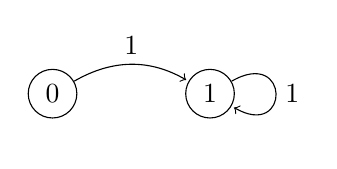
\begin{tikzpicture}[->, shorten >=1pt, scale=1, transform shape, node distance = 2cm]
    \node [circle, draw] (zero) {0};
    \node [circle, draw] (one) [right of=zero] {1};
    \path (zero) edge [bend left] node [above] {$1$} (one);
    \path (one) edge [out=30, in=-30, looseness=7] node [right] {$1$} (one);
\end{tikzpicture}
\end{center}
\end{example}

Properties:
\begin{itemize}
    \item not strongly connected
    \item aperiodic, since it has a self-loop
    \item $W=\twotwo{0}{1}{0}{1}$
    \item This graph has a unique stationary distribution $\pi = (0,1)$. Also, every random walk converges to this distribution in one step. This shows that the fundamental theorem of markov chains is not bidirectional. 
\end{itemize}

\begin{example}
\exlabel

\begin{center}
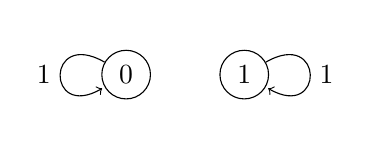
\begin{tikzpicture}[->, shorten >=1pt, scale=1, transform shape, node distance = 1.5cm]
    \node [circle, draw] (zero) {0};
    \node [circle, draw] (one) [right of=zero] {1};
    \path (zero) edge [out=150, in=210, looseness=7] node [left] {$1$} (zero);
    \path (one) edge [out=30, in=-30, looseness=7] node [right] {$1$} (one);
\end{tikzpicture}
\end{center}
\end{example}

Properties:
\begin{itemize}
    \item not strongly connected
    \item aperiodic
    \item All distributions are stationary, and therefore all walks converge to their initial distribution.
\end{itemize}

\begin{example}
\exlabel

\begin{center}
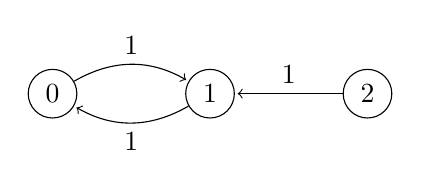
\begin{tikzpicture}[->, shorten >=1pt, scale=1, transform shape, node distance = 2cm]
    \node [circle, draw] (zero) {0};
    \node [circle, draw] (one) [right of=zero] {1};
    \node [circle, draw] (two) [right of=one] {2};
    \path (zero) edge [bend left] node [above] {$1$} (one);
    \path (one) edge [bend left] node [below] {$1$} (zero);
    \path (two) edge node [above] {$1$} (one);
\end{tikzpicture}
\end{center}
\end{example}

Properties:
\begin{itemize}
    \item not strongly connected
    \item periodic, since all cycle lengths are even
    \item there is one stationary distribution $\pi = (1/2, 1/2, 0)$
    \item there are many walks that don't converge to $\pi$. for example, any $(x,y,0)$ with $x,y\neq 1/2$ flips the mass of the first two nodes at each timestep.
\end{itemize}

\subsection{Monto-Carlo Markov Chain}

Idea: want to produce samples from a probability distribution. To do this, design a markov chain whose stationary distribution is the target distribution, and then perform samples by performing a random walk. 

\comment{not finished}

